\documentclass[a4paper]{report}
\usepackage[utf8]{inputenc}
\usepackage[T1]{fontenc}
\usepackage[english]{babel}
\usepackage{siunitx,amsmath, epic, eepic, float, subfig, amsfonts, color, amsthm, textcomp, microtype, fullpage, csquotes}
\usepackage[parfill]{parskip}
\usepackage[pdftex]{graphicx}
\graphicspath{{./assets/}}
\usepackage[titletoc,title,page]{appendix}
\usepackage{standalone}
\usepackage{array}
\usepackage{tikz}
\usepackage{pgfplots}
\usepackage{pdfpages}
\usepackage{lipsum,etoolbox}
\pgfplotsset{compat=1.14}
\usepackage{color}
\definecolor{bluekeywords}{rgb}{0.13,0.13,1}
\definecolor{greencomments}{rgb}{0,0.5,0}
\definecolor{redstrings}{rgb}{0.9,0,0}
\definecolor{light-gray}{gray}{0.95}
\usepackage[font=small,format=plain,labelfont=bf,textfont=it]{caption}
\usepackage[linkcolor=black,urlcolor=black,citecolor=black]{hyperref}
\hypersetup{colorlinks=true}
\newcommand{\HRule}{\rule{\linewidth}{0.5mm}}
\linespread{1.3}
\usepackage{beramono}
\usepackage{helvet}
\usepackage{tabulary}
\usepackage{longtable}
\usepackage{tabu}
\usepackage{todonotes}
\tabulinesep=1.2mm
\renewcommand*{\familydefault}{\sfdefault}
\renewcommand\arraystretch{1.7}
\newcommand{\code}[1]{\colorbox{light-gray}{\texttt{#1}}}
\usepackage{multirow}
\usepackage{abstract}
\usepackage[style=ieee,backend=biber,urldate=iso8601,date=iso8601]{biblatex}
\renewbibmacro*{bbx:savehash}{}
\addbibresource{references.bib}
\renewcommand{\abstractnamefont}{\normalfont\large\bfseries}
\makeatletter
\newcommand{\tocfill}{\cleaders\hbox{$\m@th \mkern\@dotsep mu . \mkern\@dotsep mu$}\hfill}
\makeatother
\newcommand{\abbrlabel}[1]{\makebox[3cm][l]{\textbf{#1}\ \tocfill}}
\newenvironment{abbreviations}{
	\begin{list}{}{
			\renewcommand{\makelabel}{\abbrlabel}
			\setlength{\itemsep}{0pt}
		}}{\end{list}
}

\usepackage{listings}
\lstdefinelanguage{JavaScript}{
  keywords={typeof, new, true, false, catch, function, =>, return, null, catch, switch, var, let, const, if, in, while, do, else, case, break, async, await, then},
  keywordstyle=\color{blue}\bfseries,
  ndkeywords={class, export, boolean, throw, implements, import, this},
  ndkeywordstyle=\color{darkgray}\bfseries,
  identifierstyle=\color{black},
  sensitive=false,
  comment=[l]{//},
  morecomment=[s]{/*}{*/},
  commentstyle=\color{purple}\ttfamily,
  stringstyle=\color{red}\ttfamily,
  morestring=[b]',
  morestring=[b]",
  morestring=[b]`
}
\lstset{frame=tb,
  language=JavaScript,
  aboveskip=3mm,
  belowskip=3mm,
  showstringspaces=false,
  columns=flexible,
  basicstyle={\small\ttfamily},
  numbers=none,
  numberstyle=\tiny\color{gray},
  keywordstyle=\color{bluekeywords},
  commentstyle=\color{greencomments},
  stringstyle=\color{redstrings},
  breaklines=true,
  breakatwhitespace=true,
  tabsize=3
}

\usepackage{longtable}
\usepackage[normalem]{ulem}
\useunder{\uline}{\ul}{}

\usepackage{titlesec}
\titleformat{\chapter}
{\normalfont\LARGE\bfseries}{\thechapter}{1em}{}
\titlespacing*{\chapter}{0pt}{3.5ex plus 1ex minus .2ex}{2.3ex plus .2ex}

\let\oldnumberline\numberline

\begin{document}

% % !TeX spellcheck = en_US
\begin{titlepage}
\begin{center}

\includegraphics[width=0.4\textwidth]{logo.pdf}~\\[1cm]

\HRule \\[0.4cm]
{ \LARGE \bfseries Functional reactive programming
	
	 in real-time web applications }\\[0.4cm]
{by Elias \textsc{Meire}}\\[0.2cm]

\HRule \\[1.5cm]

\begin{minipage}{0.49\textwidth}
\begin{flushleft} \large
\emph{Internship company:}\\
Showpad\\

\end{flushleft}
\end{minipage}
\begin{minipage}{0.49\textwidth}
\begin{flushright} \large
\emph{Supervisor:}
Rogier van der Linde\\
\emph{Mentor:}
Laurens Dewaele\\
\end{flushright}
\end{minipage}

\vfill

{\large 2016-2017}

{\large{3$^{\text{rd}}$ year bachelor Electronics-IT}}

{\large Odisee university college}

\end{center}
\end{titlepage}


% 
\includepdf{voorblad.pdf}

\newpage\null\thispagestyle{empty}\newpage


\includepdf{voorblad.pdf}


\includepdf{gegevens.pdf}

\setcounter{page}{1}
\addtocontents{toc}{\protect\renewcommand{\protect\numberline}[1]{}}

\includepdf[pagecommand={}, addtotoc={1,chapter,1,Abstract,abstract}]{abstract.pdf}
\addtocontents{toc}{\let\protect\numberline\protect\oldnumberline}

\chapter*{Acknowledgments}% (fold)
\label{sec:woord-vooraf}
\thispagestyle{plain}
\addcontentsline{toc}{chapter}{Acknowledgments}

To be written after the main content is completed.

\setcounter{tocdepth}{2}
\addcontentsline{toc}{chapter}{Contents}
\tableofcontents

\chapter*{List of Abbreviations}
\addcontentsline{toc}{chapter}{List of Abbreviations}

\begin{abbreviations}
\item[FRP] Functional reactive programming
\item[QA] Quality assurance
\item[Ajax] Asynchronous JavaScript and XML
\item[P2P] Peer-to-peer
\item[I/O] Input/output
\item[API] Application programming interface
\item[DOM] Document Object Model
\item[JSON] JavaScript Object Notation
\item[SLOC] Source lines of code
\item[JS] JavaScript
\end{abbreviations}


\newpage
\setcounter{chapter}{0}

% main content
% !TEX root = ./main.tex

\chapter{Internship company} % (fold)
\label{sec:voorstelling}

I did my internship at Showpad in Ghent. Showpad is a software as a service start-up that was founded in 2011 by ex-employees of In The Pocket, a mobile agency. Since then the company has grown at a fast pace, today Showpad has over 1000 customers and over 200 employees in offices in Ghent, London, San Francisco and Portland \cite{showpad-grow}.

Showpad provides a business-to-business service that aims to align marketing and sales departments by making marketing materials easily accessible and shareable. Showpad achieves this by hosting a platform and developing native applications for Android and iOS as well as a web application.

Showpad aims its service at enterprise customers with over 250 employees. Showpad's customers include Coca-cola, Audi, Johnson \& Johnson and many other big names \cite{showpad}. These customers pay Showpad a monthly subscription fee per user for the software as a service.

Showpad has been doubling its revenue every year for the past 4 years. At the end of 2015 Showpad's annual recurring revenue exceeded \$10 million \cite{showpad-arr}. In May 2016 Showpad closed a \$50 million funding round led by Insight Venture Partners \cite{showpad-grow}.

\section{Internal structure}

Internally Showpad is divided into 5 departments, listed in order of descending size these are: customer success, engineering, sales, marketing and employee success. As can be deduced from this order, Showpad invests heavily in customer experience. Showpad prides itself on its very short customer issue cycle time and a strong synergy between customer success and engineering is essential to achieve this.

\subsection{Engineering}

\subsubsection{Teams}

The engineering department is divided into 6 smaller teams with about 10 members. These teams are not divided by product or discipline but rather by the functionality they implement and maintain. An example of this is the create \& present team. That team maintains all user functionality related to creating and presenting content in Showpad.

The engineering teams in Showpad are discover \& measure, distribute \& collaborate, share \& personalize and create \& present. Every team consists of frontend and backend developers as well at least one quality assurance engineer and a team coach. There are also two teams that aren't linked to specific functionality. Those teams are the mobile \& learn team and the architecture team because these are two smaller teams that can't be linked to a specific user functionality. Even though these are separate teams there is still a lot of collaboration between different teams.

During my internship I was a part of the share \& personalize team. This team maintains all features related to sharing and personalizing content in all Showpad products (except the mobile apps).


\subsubsection{Guilds}

In Showpad engineering there are guilds for every development discipline. These 4 guilds are the frontend guild, the backend guild, the architecture guild and the QA guild. Every guild has a separate group chat to share interesting articles or new developments in their areas of expertise. The guilds also have a weekly meeting to talk about any topic within their field. In these meetings every guild member has the opportunity to give a presentation or workshop on something they find interesting in their discipline.

During my internship I was a part of the frontend guild. The last week of my internship I gave a presentation during the guild. The presentation was about common pitfalls in functional reactive programming and included small code recipes and demos \cite{slides}.

\subsubsection{Kanban}

Every team has a Kanban board \cite{kanban} on which they receive and create new development tickets. These tickets are then taken through a development cycle which includes a peer code review and a testing session (see figure~\ref{figure:flow}). Sometimes there are separate Kanban boards for epics. Epics are large features that typically require a long time in development and are not specific to one team. An example of an epic I took part in during my internship is the complete rewrite of the web application in Angular 2.

For distributing tickets between developers Showpad engineering uses a pull system instead of a push system. This means that developers self-assign tasks they feel comfortable working on instead of tasks being pushed to developers by a team coach.

\begin{figure}[H]
	\centering
	
\includegraphics[width=1\textwidth]{flow}
	\caption{Ticket development cycle in Showpad}
	\label{figure:flow}
\end{figure}

\subsubsection{Continuous integration}

Showpad engineering puts a lot of effort into continuous integration and deployment. The development process is largely automated (see figure~\ref{figure:workflow}). Every commit that is pushed to a git repository gets built and tested automatically by a build server. Furthermore every pull request that is approved in a code review gets deployed to a minion where it gets tested by a QA engineer. If the QA engineer approves the changes and verifies the functionality the pull request will be deployed on the staging servers. On the staging servers a last sanity check is done to ensure everything is working. If there are no issues on staging the code will be added to a release and deployed to production in cycles of about a week on average. This very fast development cycle results in a rapidly improving product and a very quick response time to customer reported issues.

\begin{figure}[H]
	\centering
	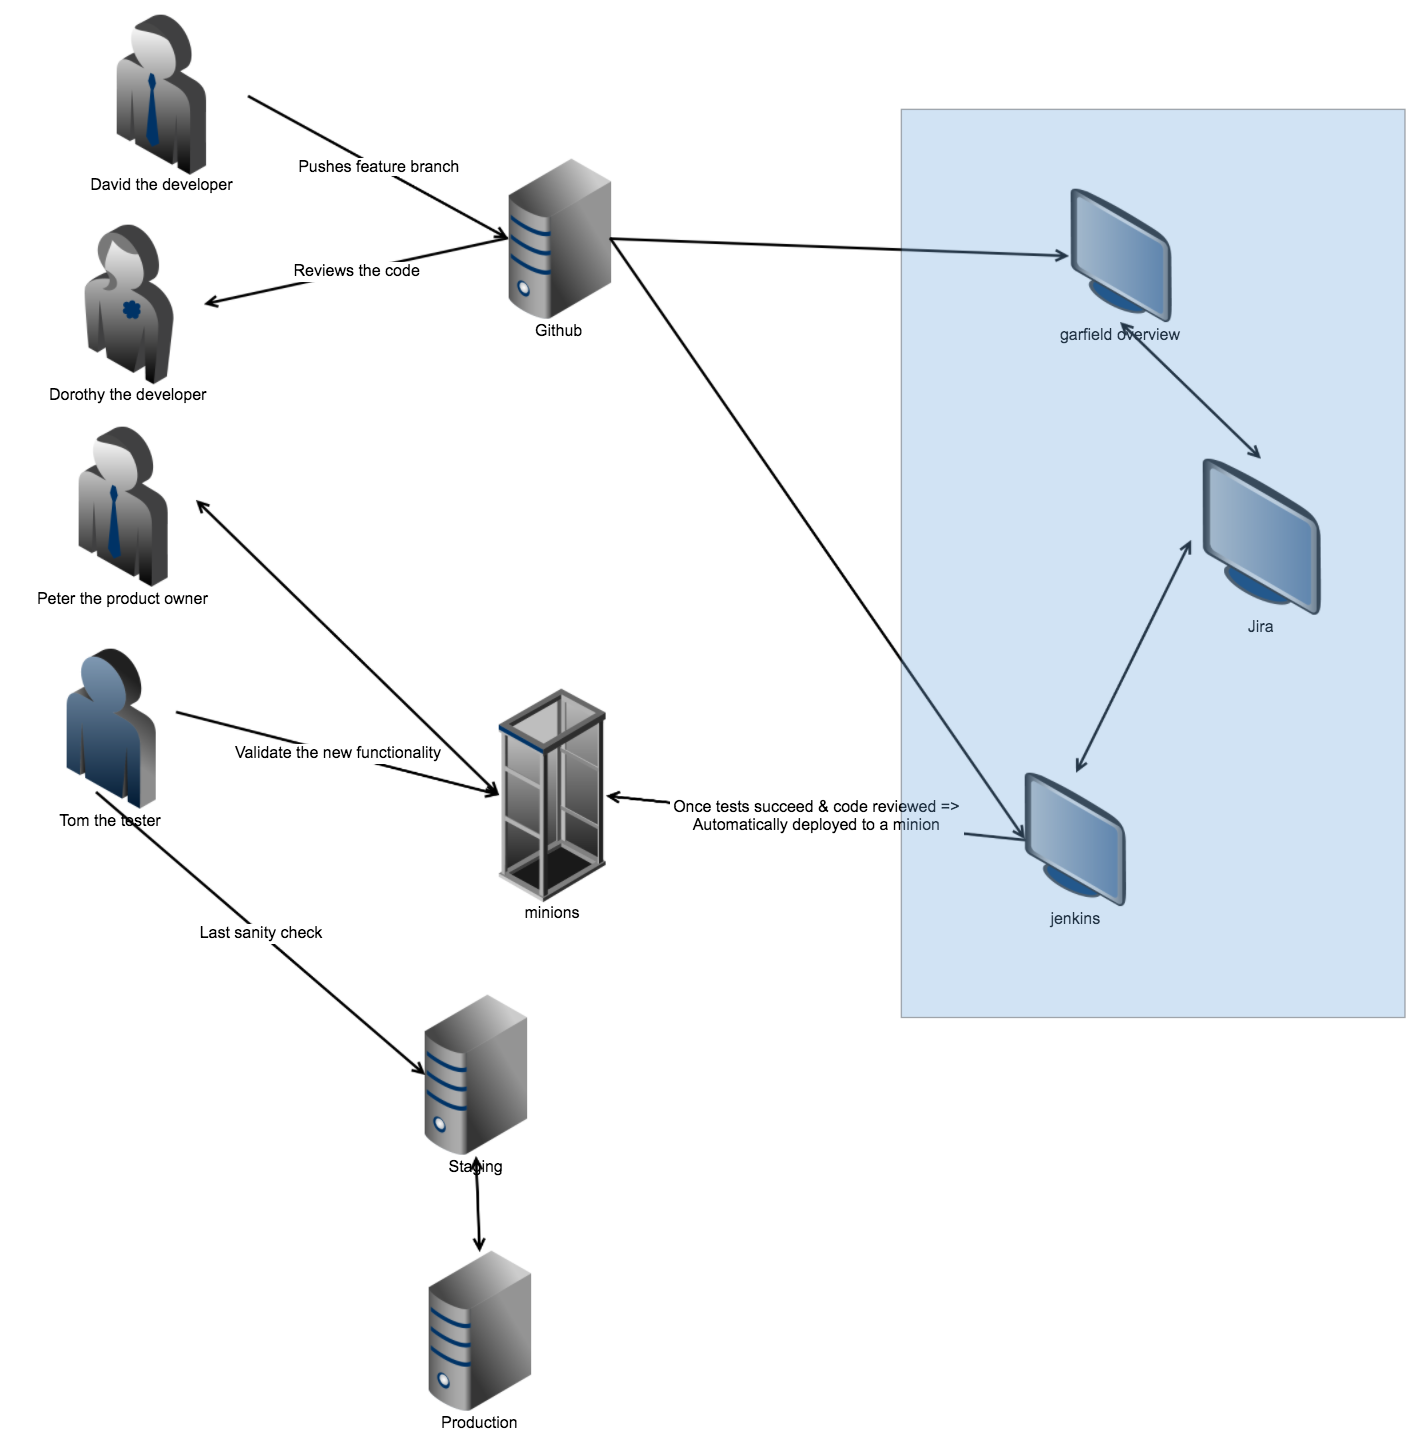
\includegraphics[width=1\textwidth]{integration}
	\caption{Showpad developer workflow diagram}
	\label{figure:workflow}
\end{figure}

\section{Culture}

Showpad has a very open culture that is typical for a start-up in the technology scene. The office is designed to be as open as possible to encourage interdepartmental collaboration and create a good atmosphere in general (see figure~\ref{figure:office}).

\begin{figure}[H]
	\centering
	
\includegraphics[width=0.9\textwidth]{office}
	\caption{Showpad office atmosphere}
	\label{figure:office}
\end{figure}

\subsection{Showings}

Showpad outlines 6 characteristics called showings that a good Showpad employee should have. These showings are shown in figure~\ref{figure:showings}.

\begin{figure}[H]
	\centering
	
\includegraphics[width=0.6\textwidth]{showings}
	\caption{The 6 showings}
	\label{figure:showings}
\end{figure}

\subsection{Events}

Showpad organizes a lot of events for its employees and customers. Every Friday evening there is an event for all employees where they can have drinks together to set off the weekend. Every other week there is also a Showpie on Friday. This is an event where all employees in all offices get together in a video call and there is a moment to ask questions to the leadership. Sometimes Showpie also includes a speech or presentation by the CEO.

Showpad engineering organizes their own yearly developer conference in Ghent called GEARS \cite{showpad-gears}. This is a free event open to all web developers. The event hosts talks and presentations by Showpad engineers and external speakers from leading technology companies. There are open donations on the event that go to a charity of Showpad's choosing.

Lastly Showpad organizes a yearly event for its customers called Showtime. Showtime gives Showpad customers a chance to share their experience with the product \cite{showpad-showtime}.





\chapter{Internship assignment} % (fold)
\label{sec:opdracht}

My internship assignment at Showpad will consist of 3 main components: the web app rewrite, speed monitor and the Showkiosk.

\section{Web app rewrite}

The largest part of my internship at Showpad will be spent doing work on the web app v2. Showpad web app v2 is a complete rewrite of the original web app in Angular 2+ and RxJS. The decision to rewrite the web app was made in July 2016 because of two major reasons. The first reason was that web app v1 was written as one big monolith. As a result development on the project was tedious, especially for new developers. The second reason is that the technologies that v1 was made with have become heavily outdated (ex. Angular 1).

During my internship I will work on the web app v2 until it gets released to customers. Afterwards I will still be part of development team on web app v2. This development will include fixing bugs and implementing new features.

\section{Web app speedmonitor}

The web app speed monitor will be a data visualisation that will measure and display the performance of the web app in real-time. Some of the technologies used in this project will be React, RxJS, Redux and Websockets. This application will be developed from scratch during my internship.

\section{Showkiosk}

The Showkiosk is an internal tool to display important message on screens throughout the company. Key technologies used in this project are Angular 2+ and Google Firebase.

\section{Relation to bachelor thesis}

The assignments in my internship are all related to the topic of my bachelor thesis. These assignments are outside the scope of this thesis but lessons learned from using the technologies on these projects will be used as a basis to understand them and write this bachelor thesis.

\chapter{Planning} % (fold)
\label{sec:actieplan}

\begin{longtable}{|l|l|l|l|}
	\hline
	\textbf{Step} & \textbf{Content}                                                                                                                                 & \textbf{Target date} & \textbf{Real date} \\ \hline
	\multicolumn{4}{|c|}{\textbf{Deadlines}}                                                                                                                                                                     \\ \hline
	1.            & Create planning & &          \\ \hline
	2.            & Decide title for bachelor thesis                                                                                                                 & 20/03                & 16/03              \\ \hline
	3.            & Submit first part of bachelor thesis                                                                                                             & 27/03                & 27/03              \\ \hline
	4.            & Intermediate evaluation by internship mentor                                                                                                     & 31/03                & 28/03                   \\ \hline
	5.            & Submit second part of bachelor thesis                                                                                                            & 24/04                &  24/04                  \\ \hline
	6.            & Submit bachelor thesis                                                                                                                           & 26/05                & 26/05                   \\ \hline
	\multicolumn{4}{|c|}{\textbf{Research}}                                                                                                                                                                      \\ \hline
	1.            & Functional Reactive programming                                                                                                                  & 20/02                & 19/02              \\ \hline
	1.            & Declarative vs. imperative programming                                                                                                           & 20/02                & 19/02              \\ \hline
	2.            & Real time on the web (Websockets, long polling...)                                                                                               & 27/02                & 28/02              \\ \hline
	2.            & Reactive implementations in Javascript                                                                                                           & 27/02                & 26/02              \\ \hline
	3.            & Elm: A purely functional language for the web                                                                                                    & 06/03                & 10/03              \\ \hline
	4.            & FRP in user interfaces                                                                                                                           & 13/03                & 13/03              \\ \hline
	4.            & Further research on FRP                                                                                                                          & 13/03                & 13/03              \\ \hline
	5.            & Matching FRP with Real-time applications                                                                                                         & 20/03                & 23/03              \\ \hline
	\multicolumn{4}{|c|}{\textbf{Internship}}                                                                                                                                                                    \\ \hline
	1.            & {\ul Web app v2 (Angular 2+, RxJS rewrite)}                                                                                                      &                      &                    \\ \hline
	& \begin{tabular}[c]{@{}l@{}}Verify existence of issues reported in v1 that are still in\\ v2 and help solving them\end{tabular}                   & 20/03                & 17/03              \\ \hline
	& Maintenance, bug fixes and improvements                                                                                                          & 12/05                & 05/05                   \\ \hline
	& Help develop new feature (Locked pages project)                                                                                                  & 12/05                &   Canceled                 \\ \hline
	2.            & {\ul Speed monitor (Websockets, React)}                                                                                                                &                      &                    \\ \hline
	& Help develop team tool to monitor speed of web app                                                                                               & 12/05                &   12/05                 \\ \hline
	3.            & { \ul Showkiosk (Angular 2+, Google Firebase)}                                                                                                          &                      &                    \\ \hline
	& \begin{tabular}[c]{@{}l@{}}Help develop Internal communication tool to display messages\\ throughout the entire company (1day/week)\end{tabular} & 12/05                & 12/05                   \\ \hline
	\caption{Planning for internship and bachelor thesis}
	\label{planning}
\end{longtable}

\chapter{Research question}

In this bachelor thesis research is conducted on how functional reactive programming can be beneficial to development of real-time web applications. The research question that is answered is the following: "What advantages and disadvantages does functional reactive programming have when developing real-time web applications?".

\section{Approach}

The first part of this bachelor thesis researches FRP and real-time dataflow on the web today. Because this bachelor thesis is applied to the web all code examples are written in JavaScript.

To come to a conclusion a practical case study is made. The research question is evaluated by implementing a simple case in a traditional imperative programming style and in a declarative FRP style. The metrics defined in section \ref{sec:metrics} will then be used to compare the two implementations and formulate a conclusion.

The case that is implemented in this bachelor thesis is a simple text-based chat application. This is the simplest example of a real-time web application with full-duplex communication.

\section{Metrics}
\label{sec:metrics}

First static analysis is performed on the source code of both implementations. Metrics that result from this analysis such as bundle size and complexity metrics are then used to compare the implementations. After that the runtime performance of both implementations is compared in two scenarios. Finally there is a comparison based on the readability of the source code.

\chapter{Real-time on the web} % (fold)
\label{sec:realtime}

\section{HTTP Polling} % (fold)
\label{sub:polling}

The simplest way to do real-time on the web is to poll a server via Ajax at a certain interval. This is a simple but very primitive way to update data in real-time. This technique has multiple downsides. Firstly the communication is not really real-time and your data is always out of date because of the usage of an interval. Secondly this technique increases load on your server because it has to handle a lot of requests from the clients. This makes scaling with an HTTP polling architecture very cumbersome \cite{poll-socket}. Lastly this technique cannot do two-way communication between server and client so it is not suitable for real-time communication \cite{poll-socket}.

\section{HTTP long polling} % (fold)
\label{sub:long-polling}

HTTP long polling is a variation on HTTP polling. The client still polls the server for new data but the server keeps the request open until it has new data. After the client gets a response it immediately sends a new request, repeating the process \cite{long-poll} (see figure~\ref{figure:long-poll}). This technique resolves most downsides of classic HTTP polling but it still cannot facilitate two-way communication between server and client \cite{poll-socket}.

\begin{figure}[H]
	\centering
	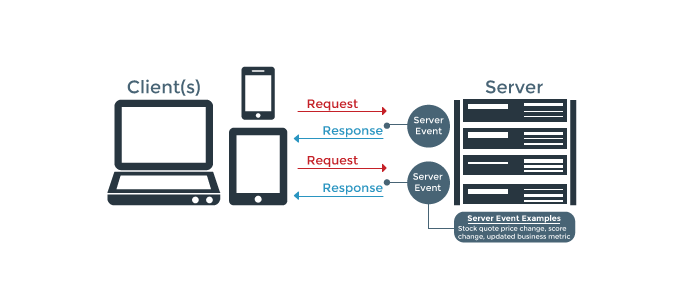
\includegraphics[width=1\textwidth]{long-poll}
	\caption{Long polling \cite{long-poll}}
	\label{figure:long-poll}
\end{figure}

\section{WebSockets} % (fold)
\label{sub:websockets}

HTML5 WebSockets are a full-duplex communication channel (see figure~\ref{figure:socket}) that operates through a single socket over the web. HTML5 WebSockets are not just another small improvement over conventional HTTP communications \cite{poll-socket}, it is a completely new communication protocol. Under the hood WebSockets are built on TCP; they do not use HTTP except for establishing the connection \cite{socket-wiki}. Browser support for WebSockets is excellent, all major browsers support them \cite{socket-browser}.


\begin{figure}[H]
	\centering
	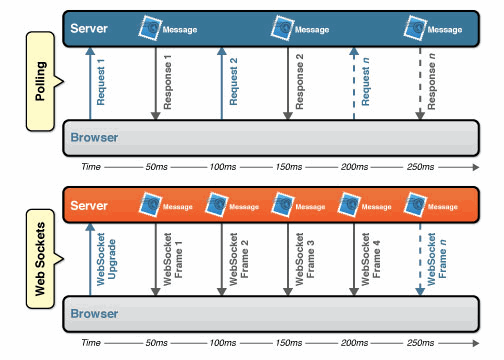
\includegraphics[width=0.8\textwidth]{socket}
	\caption{Comparison of HTTP polling and WebSockets \cite{poll-socket}}
	\label{figure:socket}
\end{figure}

\subsection{Libraries} % (fold)
\label{sub:websockets-implementations}

There are many libraries that abstract away some of the complexity from the WebSocket protocol. The most popular WebSocket libraries at the time of writing are Socket.IO, Primus, ws and Faye. The most popular reasons to choose a library over using the vanilla version are elegant fallbacks for browsers that do not support WebSockets and automatic reconnection.

\section{WebRTC} % (fold)
\label{sub:webrtc}

WebRTC is a full-duplex communication protocol that was developed and open sourced by Google in 2010 \cite{webrtc-intro}. After that WebRTC was standardised by the IETF and the W3C \cite{webrtc-intro}. Now there are implemented open standards for real-time, plugin-free video, audio and data communication. WebRTC allows real-time peer-to-peer communication of audio, video and arbitrary data between browsers. A server is only needed to set up the initial connection between peers, this process is called signaling \cite{webrtc} (see figure~\ref{figure:signal}).

\begin{figure}[H]
	\centering
	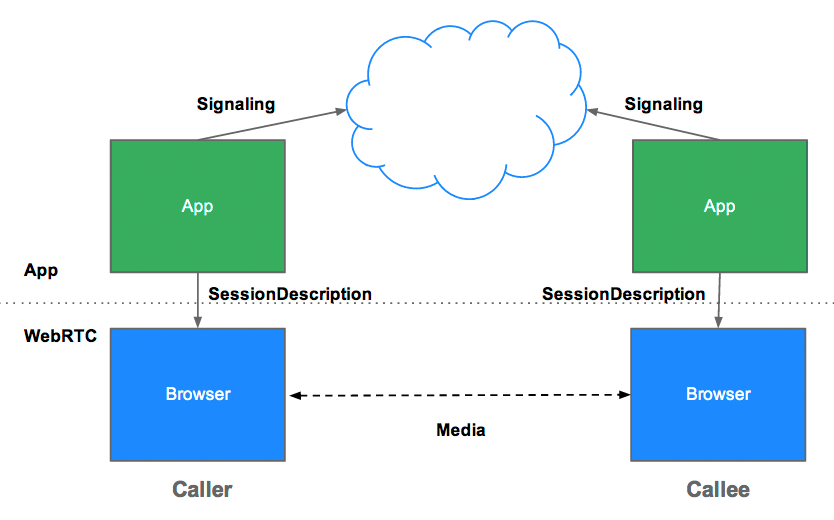
\includegraphics[width=0.8\textwidth]{signal}
	\caption{Signaling process for WebRTC \cite{webrtc-intro}}
	\label{figure:signal}
\end{figure}

WebRTC's P2P connection model further increases scalability and simplicity of real-time applications \cite{webrtc}. However WebRTC also has some caveats. Even though it has been around for 4 years now browser support is still lacking at the time of writing \cite{webrtc-browser}. It is also hard to implement WebRTC in a client-server architecture \cite{hn} as it was primarily made for P2P communication.

\chapter{Functional reactive programming} % (fold)
\label{sub:frp}

Functional reactive programming is a programming paradigm that integrates the idea of asynchronous dataflows into functional programming. This provides an elegant way to express computation for areas that involve a lot of time related variables such as animation and user interface rendering \cite{frp-wiki}\cite{frp-haskell}. 

\section{Functional programming} % (fold)
\label{sub:fp}

Functional programming is a programming paradigm that models computation as a composition of pure functions without mutating any state \cite{func-js}. It is a declarative programming paradigm. One of the biggest advantages of functional programming is that by using pure functions it becomes much easier to reason about the behavior of a program \cite{func-js}.

Functional programming has its origins in lambda calculus, a system in mathematical logic for expressing computation based on operations and variables \cite{lambda}.

\subsection{Declarative programming}

In declarative programming a program describes what to do, rather than how to do it. This is the opposite of traditional imperative programming \cite{intro-func}. The difference between the two is best explained by example. Listing~\ref{listing:imp} and listing~\ref{listing:dec} both show an implementation of a function called \code{double()}. The function takes an array and returns another array with all elements doubled. Listing~\ref{listing:imp} shows an imperative implementation of this function, the function explicitly says to loop over the elements, double them and add them to an empty array. Listing~\ref{listing:dec} shows a declarative implementation of this function, it only says what we want to happen to the elements in the array.

\begin{lstlisting}[caption=Imperative implementation of the double function,label=listing:imp]
function double (arr) {
	let results = [];
	for (let i = 0; i < arr.length; i++) {
		results.push(arr[i] * 2);
	}
	return results;
}
\end{lstlisting}

\begin{lstlisting}[caption=Declarative implementation of the double function,label=listing:dec]
function double (arr) {
	return arr.map(item => item * 2);
}
\end{lstlisting}


\subsection{First-class functions}

In functional programming functions are first-class citizens. This means that functions can be treated like any other value. They can be created, stored in data structures and passed into or returned from other functions.

\subsubsection{Pure functions}

Pure functions have two defining characteristics. The first is that the function's result only depends on its arguments, given the same arguments the function always returns the same value \cite{intro-func}. The second characteristic is that pure functions do not cause any side effects such as mutations to data structures or output to I/O devices \cite{intro-func}.

\subsubsection{Higher order functions} % (fold)
\label{sub:fp-order}

Higher order functions are functions that either take a function as an argument, return a function or both. This is a simple concept that makes function composition possible. Function composition helps to keep functional programs readable and easy to reason about \cite{intro-func}.

An example of a higher order function in JavaScript is the \code{map()} function of the Array prototype (see listing~\ref{listing:dec}). This function takes another function as its argument. The \code{invokeTwice()} function in listing~\ref{listing:ho} is an example of a higher order function that returns a function.

\begin{lstlisting}[caption=Higher order function composition,label=listing:ho]
const invokeTwice = f => subject => f(f(subject));
const double = x => x * 2;
const quad = invokeTwice(double);

quad(10); // 40
invokeTwice(double)(10); // 40
\end{lstlisting}

The \code{invokeTwice()} function takes a function as an argument and returns a function that applies the first function twice on its argument. The example also shows how \code{invokeTwice()} can be composed together with other functions such as \code{double}. A function like \code{invokeTwice()} that takes one argument at a time and returns a function taking the next argument is called a curried function. \cite{func-js}.

\subsection{Immutability}

Functional programming promotes the use of immutable data structures, most functional languages even enforce it \cite{func-js}. Immutability means that a data structure cannot be changed. If an operation is done on an immutable object, it copies the value, mutates it and returns it as a new object. This helps eliminate bugs where an object enters a state that was not predicted by the programmer \cite{intro-func}.

\subsection{Other functional jargon}

There are many other terms associated with functional programming but these are out of scope for this thesis. This chapter only serves to give a basic understanding of the functional programming paradigm.

\section{Reactive programming}
\label{sub:rp}

Reactive programming is a programming paradigm that deals with asynchronous data streams \cite{intro-reactive}. These data streams then propagate their changes to other parts of the application; this is the observer pattern \cite{observer}. Reactive programming has three main objects: an observable or a stream, an observer or a subscriber and a scheduler \cite{intro-reactive}.

An observable emits values over time. An observable can be infinite or it can complete after a certain number of emitted values. Observers can subscribe to these streams and get notified whenever the observable emits a value, throws an error or completes (see listing~\ref{listing:observer} for an example). Schedulers decide on which thread an observer's code should run and when.

\begin{lstlisting}[caption=An observable and observer in RxJS,label=listing:observer]
const someObservable$ = Observable.from([1,2,3]);

someObservable$
	.subscribe(
		value => console.log(value),
		error => console.err(error),
		completed => console.log('completed')
	);
	
// output: 1, 2, 3, completed
\end{lstlisting}

\subsection{Operators}

Typically an FRP library or language includes a lot of operators \cite{intro-reactive} so that observables can be easily manipulated. In FRP operators are pure functions that take an observable and return another observable. A simple example of an operator is the delay operator. This operator is available in RxJS and returns the input observable with every value delayed by a specified amount of time \cite{delay} (see figure~\ref{figure:delay}). Because operators return a new observable, operators can be easily chained after one another.

\begin{figure}[H]
	\centering
	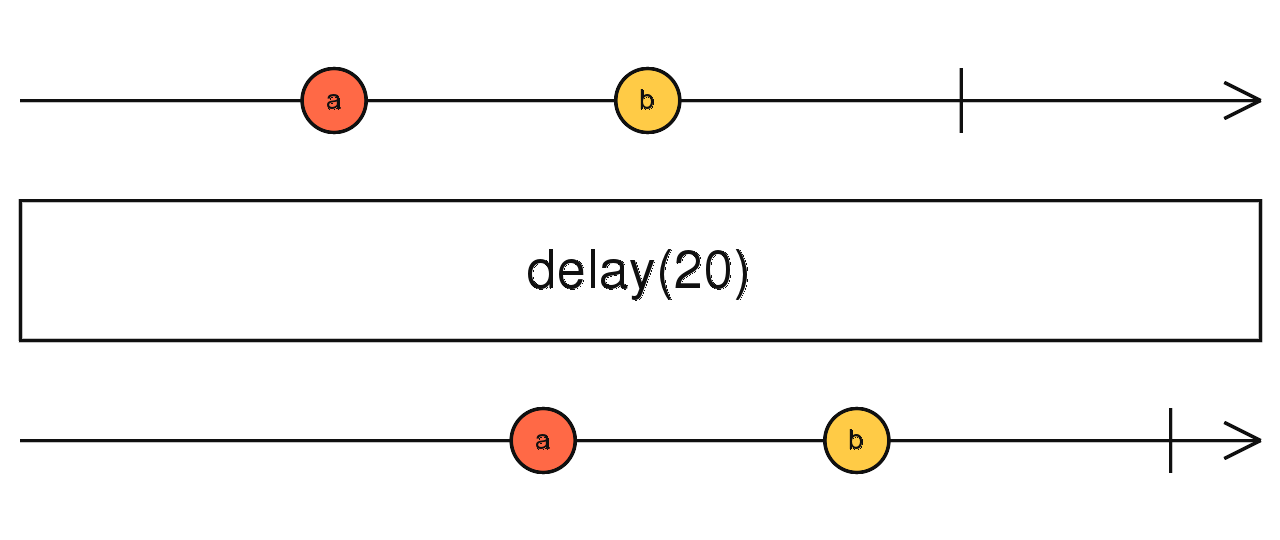
\includegraphics[width=0.7\textwidth]{delay}
	\caption{The delay operator in RxJS: marble diagram \cite{delay}}
	\label{figure:delay}
\end{figure}

An example of operators on a data stream can be seen in figure~\ref{figure:stream}, this example illustrates a stream of clicks by a user. The events in the stream are first grouped by throttling them for 250ms. Afterwards they are mapped to the length of the groups and finally they are filtered so that only groups of clicks equal or larger than 2 remain. This example shows really well how reactive programming helps with handling complex operations on events in modern applications.

\begin{figure}[H]
	\centering
	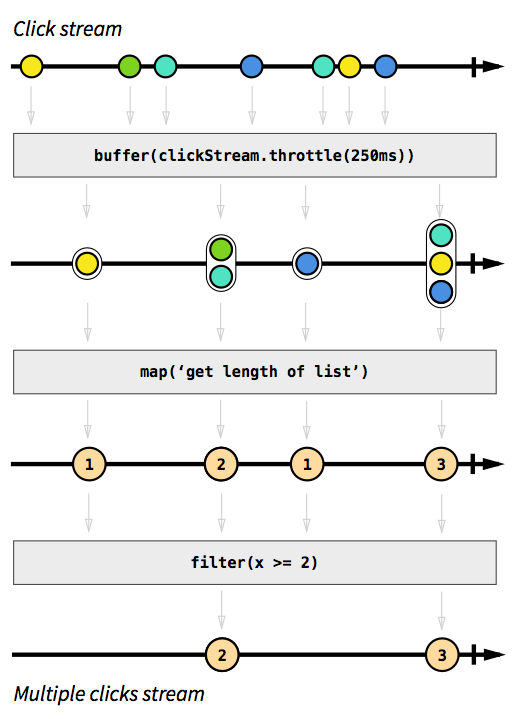
\includegraphics[width=0.5\textwidth]{stream}
	\caption{Stream of clicks \cite{intro-reactive}}
	\label{figure:stream}
\end{figure}

\subsection{Visualizing observables}

The biggest roadblock in adoption of reactive programming by developers has been the steep learning curve. Reactive programming forces the developer to think about dataflow in a different way. In reactive programming data arrives over time and is immutable. Essential in learning to think reactive is being able to visualize how observables work over time.

Marble diagrams are the main tool that is used today to visualize observables. These diagrams can be great tools to not only understand the core concepts of reactive programming but also understand the functionality of individual operators (see figure~\ref{figure:delay} and \ref{figure:stream}).

\subsection{Debugging}

The main area where reactive programming falls short today is debugging. Since operators tend to be one line arrow functions it is not possible to set a breakpoint inside them. This results in a lot of developers either using console statements or having to convert operator functions to functions with a body every time they want to debug. Moreover stack traces tend to be longer and less useful than those from imperative programming. Because everything is asynchronous and a lot of work is done internally in the FRP library, stack traces tend to show only the errors internal to the library which is not useful for the developer \cite{debug}. An important side note is that Paul Irish announced new features coming to Chrome Devtools during Google I/O 2017 that will allow developers to debug asynchronous code more efficiently \cite{devtools}. Stack traces will become more descriptive and developers will be able to step inside one line arrow functions such as \code{Promise.then()} \cite{devtools}.

RxJS 5 is a complete rewrite of RxJS 4 and one of its biggest improvements is its shorter stack traces making it easier for developers to debug their code \cite{debug}. Other tools one can use to debug and reason about reactive code are marble diagrams and dependency graphs \cite{debug}. Marble diagrams let developers visualize observables and find mistakes in their reasoning. Dependency graphs help the developer understand what observables an observable depends on and for what. This helps identify problems where an observable the current observable depends on is not behaving the way the developer expects it to. An example of a dependency graph is shown in figure~\ref{figure:depgraph}.

\begin{figure}[H]
	\centering
	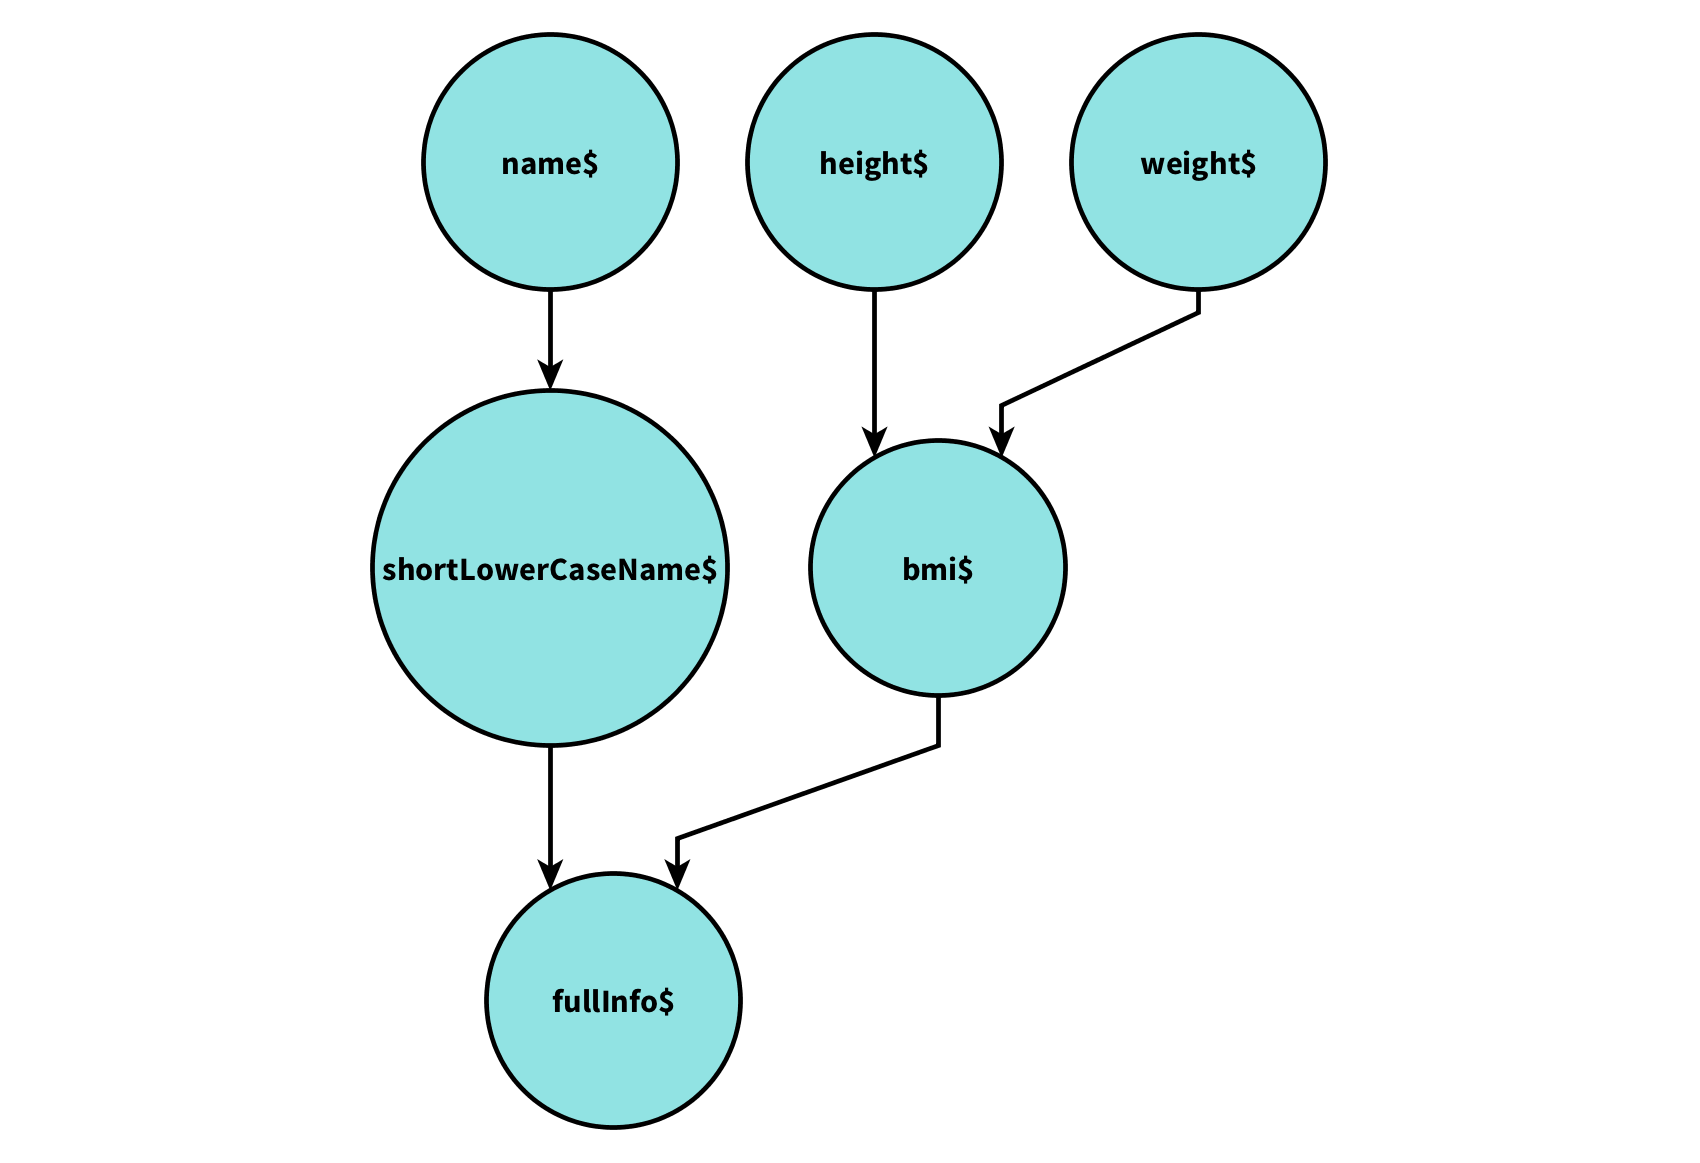
\includegraphics[width=0.9\textwidth]{dep}
	\caption{A dependency graph of observables in a BMI calculator \cite{debug}}
	\label{figure:depgraph}
\end{figure}

Figure~\ref{figure:depgraph} above shows the dependency graph of a simple Body Mass Index (BMI) calculator. The code associated with this example can be seen in listing~\ref{listing:bmi}. The code example assumes that the input streams \code{name\$}, \code{weigth\$} and \code{height\$} are already instantiated before this code runs. 

\begin{lstlisting}[caption=Reactive BMI calculator source code \cite{debug},label=listing:bmi]
const shortLowerCaseName$ = name$
	.map(name => name.toLowerCase())
	.filter(name => name.length < 5);

const bmi$ = weight$
	.combineLatest(
		height$,
		(weight, height) => Math.round(weight / (height * height * 0.0001))
	);

const fullInfo$ = shortLowerCaseName$.combineLatest(bmi$);
\end{lstlisting}

\subsection{Hot and cold observables}

Observables can be either hot or cold. The way the producer is linked with the observable defines whether it is hot or cold. A producer is an object that provides values to an observable. The producer can be an iterator, an event, a WebSocket etc. The pseudocode in listing~\ref{listing:hot} shows how a producer is linked up to an observable for hot and cold observables.

\begin{lstlisting}[caption=Hot and cold observables in RxJS \cite{hot},label=listing:hot]
// Cold observable
const cold = new Observable((observer) => {
	const producer = new Producer();
	// have observer listen to producer here
});

// Hot observable
const producer = new Producer();
const hot = new Observable((observer) => {
	// have observer listen to producer here
});
\end{lstlisting}

When creating a cold observable a producer is made for each observer. This means that if there is no observer subscribed there is also no producer being instantiated. This is the reason why observables in RxJS need to be subscribed to in order to emit anything at all. Cold observables are unicast \cite{hot}. This means that every producer only emits its data to one observer. As a result this can cause issues when working with very rapidly changing data such as time. Because every observer has its own producer, the time at which observers receive the same data can differ slightly \cite{hot}.

For a hot observable the producer is set up even if no observer is subscribed to it. When multiple observers subscribe to the same observable the producer is shared. Emitted data from the producer is multicasted to all observers \cite{hot}. In most FRP libraries including RxJS, observables are cold by default. Observables in RxJS can be made hot with the publish and share operators \cite{hot}, subjects (see section~\ref{subjects}) are always hot.

\subsection{Subjects} \label{subjects}

Subjects are an additional data structure provided in some FRP libraries. Subjects behave exactly like observables but their data does not come from a producer. Instead data can be pushed manually to the subject \cite{subjects}. This helps bridge the gap between imperative programming and reactive programming. Subjects make it easy for a programmer to integrate stateful data into an observable. Since subjects are compatible with all observable operators they can be combined with other observables. It is considered to be a bad practice though and whenever it can be avoided it is advised to use observables over subjects \cite{subjects}.

\section{FRP in JavaScript}

Because of JavaScript's unopinionated nature, choice of programming paradigm is left to the developer. JavaScript also has a lot of the ingredients needed for FRP built into the language. Functions in JavaScript are already first-class citizens of the language \cite{func-js}. Arrow functions allow JavaScript functions to be reasoned about as lambda calculus and finally ES2015 introduced a few functional array functions such as map, reduce and filter \cite{es2015}.

Because of these characteristics JavaScript is an excellent language for functional reactive programming.

\subsection{Asynchronous Javascript}

Dealing with asynchronous code has always been one of the biggest challenges of programming for the web. Over the years developers have employed different techniques to handle asynchronous code in JavaScript.

\subsubsection{Callbacks}

Callbacks are the simplest way to handle asynchronous code in JavaScript. The principle is simple; a callback function is passed as an argument with another function. That function will then call the callback function when it finishes its work.

The problem with callbacks is that they quickly become unreadable when the programmer needs to compose different asynchronous actions. Listing~\ref{listing:cb} is an example of 3 asynchronous functions running one after the other. This example code is already pretty complex even though it accomplishes a very simple task.

\begin{lstlisting}[caption=Fetching data  with nested callbacks,label=listing:cb,float]
getData(function (err, x) {
	if(err) {
		console.error(`Oh no! an error: ${err}`);
		return;
	}
	getMoreData(x, function (err, y) {
		if(err) {
			console.error(`Oh no! an error: ${err}`);
			return;
		}
		other(x, y, function (err, z) {
			if(err) {
				console.error(`Oh no! an error: ${err}`);
				return;
			}
			...
		});
	});
});
\end{lstlisting}

\subsubsection{Promises}

Promises are an alternative way to handle asynchronous code. Promises were standardized in ES2015 but have been around for years in various libraries such as Bluebird \cite{promise}. The Promise API allows the developer to compose asynchronous code in a more declarative manner. A promise can either resolve and deliver a value or reject and throw an error.

Listing~\ref{listing:promise} shows the example of listing~\ref{listing:cb} rewritten with the JavaScript Promise API. The \code{Promise.catch()} function handles all errors on a chain of promises.

\begin{lstlisting}[caption=Fetching data with the Promise API,label=listing:promise]
getDataPromise
	.then(x => getMoreDataPromise(x))
	.then(y => otherPromise(y))
	.then(z => ...)
	.catch(err => {
		console.error(`Oh no! an error: ${err}`);
	});
\end{lstlisting}

If the promises in the example would not depend on the result of the previous one the \code{Promise.all()} function could be used. This function completes when all promises have resolved. The \code{Promise.all()} function throws an error if one of the promises rejects \cite{prom-all}.

\subsubsection{Async/await}

Async functions and the async/await syntax was recently introduced to JavaScript in ES2017 \cite{async-await}. It is a new language construct to handle asynchronous code. The await keyword blocks code execution until an async function has completed. The example used in listing~\ref{listing:cb} and listing~\ref{listing:promise} is rewritten below in listing~\ref{listing:await} using the async/await syntax. 

\begin{lstlisting}[caption=Fetching data with the async/await keywords,label=listing:await]
async function getAllData() {
	try {
		const x = await getData();
		const y = await getMoreData(x);
		const z = await other(y);
		...
	} catch(err) {
		console.error(`Oh no! an error: ${err}`);
	}
}	
\end{lstlisting}

\subsubsection{Functional Reactive Programming}

FRP provides a more versatile API to handle asynchronous code than Promises and async/await. As Akash Agrawal correctly notes in his article "What Promises Do That Observables Can’t" observables completely overshadow promises in terms of functionality \cite{observables-promises}.

Listing~\ref{listing:observable-getdata} shows the example from the listings in the previous paragraphs rewritten using RxJS observables. The \code{getMoreDataObservable()} and \code{getOtherObservable()} functions in this example return an observable based on their parameter. While the implementations with promises and async/await are slightly more concise, FRP offers a lot more functionality than both. RxJS observables for example provide operators to cancel, buffer and debounce asynchronous code \cite{rxjs-ben}. Promises or async/await provide no API for those functionalities.

\begin{lstlisting}[caption=Fetching data with FRP (RxJS),label=listing:observable-getdata]
dataObservable$
	.flatMap(x => getMoreDataObservable(x))
	.flatMap(y => getOtherObservable(x))
	.catch(err => {
		console.error(`Oh no! an error: ${err}`);
	})
	.subscribe(z => {
		...
	});
\end{lstlisting}

\subsection{Current state}

Many libraries already bring FRP to JavaScript. The most popular ones at the time of writing are RxJS, xstream and Bacon.js \cite{intro-reactive}. There is also a proposal out there to bake an observable data structure into a future version of ECMAScript \cite{tc39}.

In 2013 Evan Czaplicki and Stephen Chong published a thesis at the Harvard University about the creation of Elm \cite{elm}. Elm is a practical FRP language with two important features: high-level abstractions to support simple, declarative FRP and purely functional graphical layout calculation \cite{elm}. Elm is also known for its excellent tooling and the absence of runtime errors in the language. Most importantly the Elm language is built on top of JavaScript and is made with the web in mind.

The FRP paradigm has been around for a very long time but it is still very new to the web platform. The need for a good abstraction to handle asynchronous code can be a driving factor to increase adoption of FRP in JavaScript. Possible support for observables in the JavaScript language can also further increase developer adoption in the future.



\chapter{Case study: FRP in real-time data flows} % (fold)
\label{sec:uitwerking}

In this chapter a real-time chat application is developed and analyzed. The chat application is implemented twice in different programming styles. The first implementation uses FRP for all application logic and Cycle.js to render this to the Document Object Model. The second implementation uses imperative programming for all application logic and JQuery for DOM manipulation.

The backend implementation is the same for both frontend implementations. Real-time communication between server and client is implemented using WebSockets. WebSockets was chosen over HTTP long polling because long polling does not implement a full-duplex communication channel. WebSockets were chosen over WebRTC data channels because of browser support and maturity of the protocol. Furthermore WebRTC is primarily meant for P2P applications and is cumbersome to implement in a client-server application model.

The source code of this application is open source and is available on GitHub \cite{chat-code}. Excerpts from the source code will be included throughout this chapter to explain implementation details. 

\section{Interface}

The application features a very simple interface (see figure~\ref{figure:chat}). Users can enter their name and a message in the text inputs in the bottom bar. They can then click send to send a new message over the WebSocket. The server will then broadcast this message to all other clients connected to the WebSocket. 

On the frontend the messages are displayed with an avatar next to them that is automatically generated from the username of the sender. The side the messages are rendered on is dependent on whether the current user is equal to the sender of the message. A user's own messages will appear on the right and messages from other people will appear on the left.

\begin{figure}[H]
	\centering
	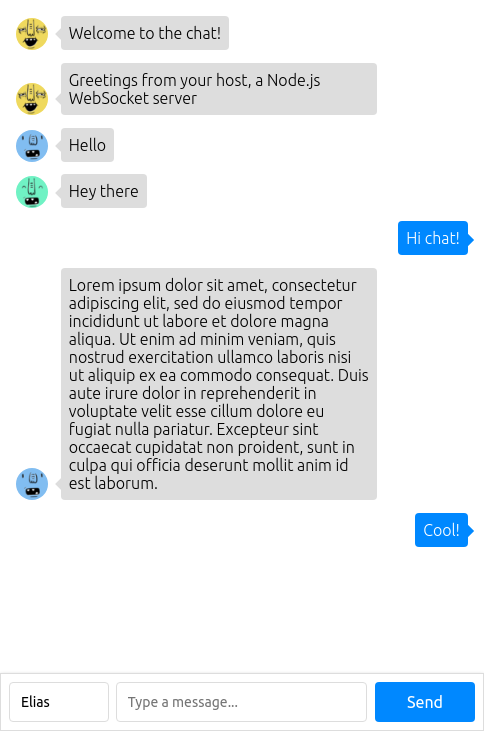
\includegraphics[width=0.6\textwidth]{chat}
	\caption{The chat application interface}
	\label{figure:chat}
\end{figure}

\section{Backend}

\subsection{Implementation}

The backend is implemented in Node.js. It makes use of the Express framework to set up an HTTP server and host the static files from the frontend. The WebSocket implementation used is µWebSockets. µWebSockets is a lightweight WebSocket implementation written in C++ with simplicity, performance and scalability as its main objectives \cite{uws}.

µWebSockets was chosen because of its simplicity and performance. This application is meant to be a very minimal implementation of a chat application and as a result it does not need any extra features on top of the WebSocket protocol. Socket.IO or other popular WebSocket libraries would have been overkill for this application as it does not need any of the extra features it provides.

Messages are not persisted on the server because it would add extra dependencies and potential performance bottlenecks. This case study is focused on the comparison of FRP and imperative programming for the web. As a result it was attempted to add as little dependencies as possible to focus on that comparison.

\subsection{Functionality}

The backend sets up the WebSocket using µWebSockets and listens for connections. When a client connects to the WebSocket the server sends out a welcome message. When a client sends a message over the WebSocket the server will broadcast this message to all clients that are currently connected.

\section{Frontend with FRP}
\label{sec:imp-frp}

\subsection{Choice of technologies}

\subsubsection{FRP library}

RxJS is used as the FRP library for this application. This choice is made mainly because of the popularity of the library. ReactiveX is a very mature cross-language FRP library with big companies like Microsoft and Netflix backing it and using it in their own applications \cite{rx}. The JavaScript version of ReactiveX (RxJS) is currently the most popular FRP library for JavaScript by a large margin. The npm installation statistics support this statement \cite{rx-npm}\cite{most-npm}\cite{xs-npm}.

Xstream and most.js were also considered. Both these FRP libraries feature better performance than RxJS and are only a fraction of the size \cite{rx-npm}\cite{most-npm}\cite{xs-npm}. But ultimately the performance and bundle size of this application is not the priority. Using RxJS has the advantage of more people being familiar with its concepts and operators.

\subsubsection{DOM abstraction}

For a DOM abstraction various frameworks and libraries are considered. Since the objective is to use FRP in the application, frameworks that play nice with FRP have the advantage. Angular is the first framework that comes to mind in this category. Angular has built-in support for observables and even uses RxJS internally for its core API's. But because of the size and complexity of Angular there is too much overhead for this application. This application is meant to be as minimal as possible and Angular does not fit the bill in that department.

Cycle.js is the next framework to be considered. Cycle.js is a functional and reactive JavaScript framework for predictable code \cite{cycle} written by André Staltz who is also a core contributor to RxJS and the author of xstream \cite{staltz}\cite{xs-npm}. Cycle.js features a very minimal API and allows the programmer to see the application as a pure function. To use Cycle.js the programmer has to only import one function \code{run()}. This makes code easy to understand for newcomers since there are no new framework API's to learn. Cycle.js is also FRP library agnostic and thus allows the programmer to use their library of choice.

Because of its minimal API and very functional architecture Cycle.js was chosen as the DOM abstraction for this application. The architecture used in Cycle.js is further explained in  section~\ref{sec:arch}.


\subsection{Architecture}
\label{sec:arch}

Cycle.js lets the developer see the app as a pure function. This \code{main()} function takes source streams as an argument and returns sink streams. Figure~\ref{figure:cycle} shows a diagram of how this architecture works in practice.

\begin{figure}[H]
	\centering
	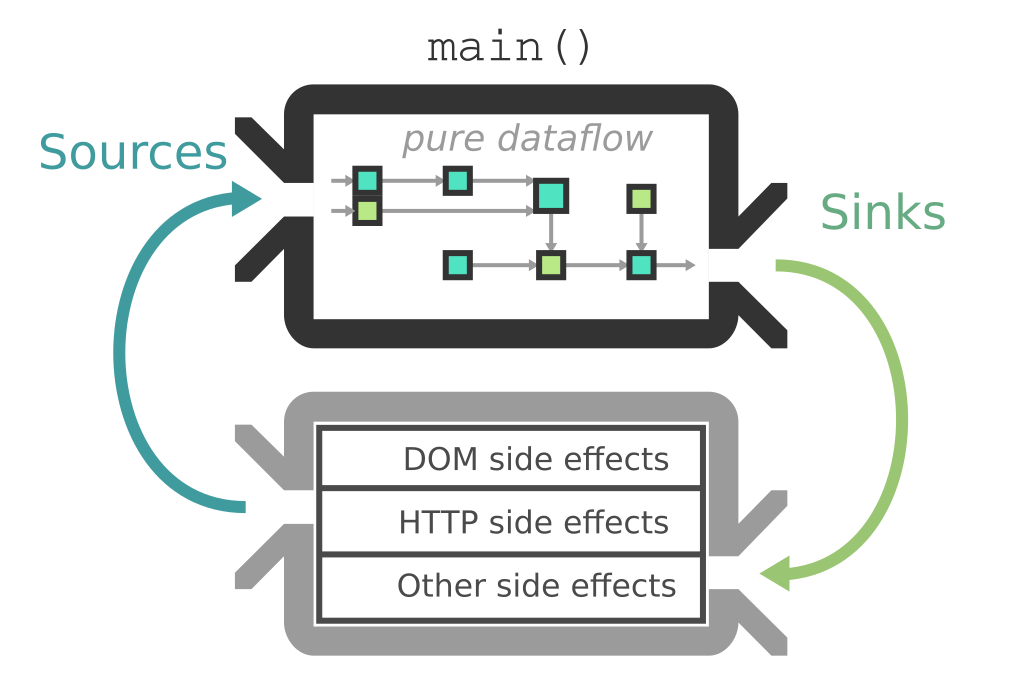
\includegraphics[width=0.8\textwidth]{cycle}
	\caption{Cycle.js application architecture \cite{cycle}}
	\label{figure:cycle}
\end{figure}

The bottom function shown in figure~\ref{figure:cycle} is called a driver. Drivers handle side effects towards various outputs such as the DOM. Drivers take sinks as an argument and return sources for the main function to use \cite{cycle-drivers}. Driver functions can be seen as the inverse of the \code{main()} function. Cycle.js provides a few basic drivers for the DOM and for HTTP requests. Cycle.js is very extensible \cite{cycle-drivers} and as a result other drivers written by the community can be found on open source platforms.

\begin{figure}[H]
	\centering
	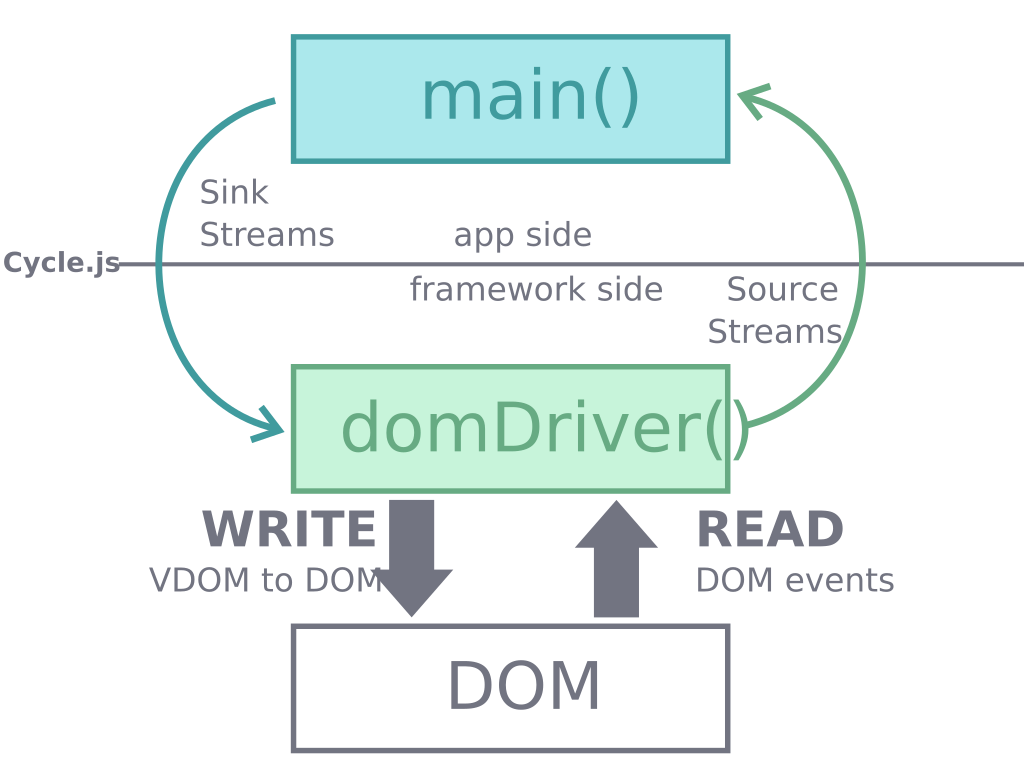
\includegraphics[width=0.7\textwidth]{driver}
	\caption{Cycle.js DOM driver diagram \cite{cycle-drivers}}
	\label{figure:driver}
\end{figure}

The diagram shown in figure~\ref{figure:driver} is an example of a Cycle.js driver. It represents the built-in DOM driver. This driver handles writing DOM changes from the sink stream and provides DOM elements and events in the source stream.

\subsubsection{Custom WebSocket driver}

For this project a custom driver was developed to set the WebSocket up as a source and a sink stream. The driver is available as a package on npm \cite{driver-npm} so that it can be used by other users of Cycle.js. The source code is open source and is available on GitHub \cite{driver-github}.

The driver is a wrapper around the WebSocketSubject object provided by RxJS \cite{ws-subject}. Internally the driver acts as an adapter that forwards the messages from the sink stream to the WebSocketSubject. The driver returns the WebSocketSubject as a whole as a source stream, that way the developer has full control over it in the \code{main()} function. Special attention was given to ensure that the driver is also compatible with other FRP libraries such as xstream and Most.js.

\subsection{Implementation}

When developing an application with the concept of source and sink streams the developer first defines the input streams needed for the application. These input streams can be user input, a real-time database etc.

In the case of this application these input streams will be inputs from the user through DOM events and messages from the WebSocket. In the source code the input streams are defined as in listing~\ref{listing:input-streams}. The input streams are derived from the sources given as an argument to the Cycle.js \code{main()} function. In some cases the input streams might even be just a source without any mutation.

The \code{scan} operator on the WebSocket source collects all messages received up until this point in an array. The marble diagram in the comment on line 2 shows how this works in practice. \code{\{m\}} represents a single message object.

\begin{lstlisting}[caption=Definition and instantiation of the input streams,label=listing:input-streams]
const messages$ = ws.scan((acc, m) => [...acc, m], []);
// --[]--[{m}]--[{m}, {m}]--[{m}, {m}, {m}]-->
const formSubmit$ = DOM.select('#form').events('submit');
const senderInput$ = DOM.select('#sender').events('input');
const messageInput$ = DOM.select('#message').events('input');
\end{lstlisting}

After the input streams are defined the developer can think about what sinks (output streams) the application will output towards. In the case of web applications one sink that will always be used is the DOM. LocalStorage is an example of another output stream that some applications use. In the case of this application the used sinks are the DOM and the WebSocket.

Now that the sources and sinks are known all that is left to do is to combine and manipulate the input streams until they are in the required format for the sinks. Before writing any code it can be useful for the developer to make a dependency graph to see which output streams depend on which input streams. The dependency graph for this chat application is shown in figure~\ref{figure:chat-dep}.

\begin{figure}[H]
	\centering
	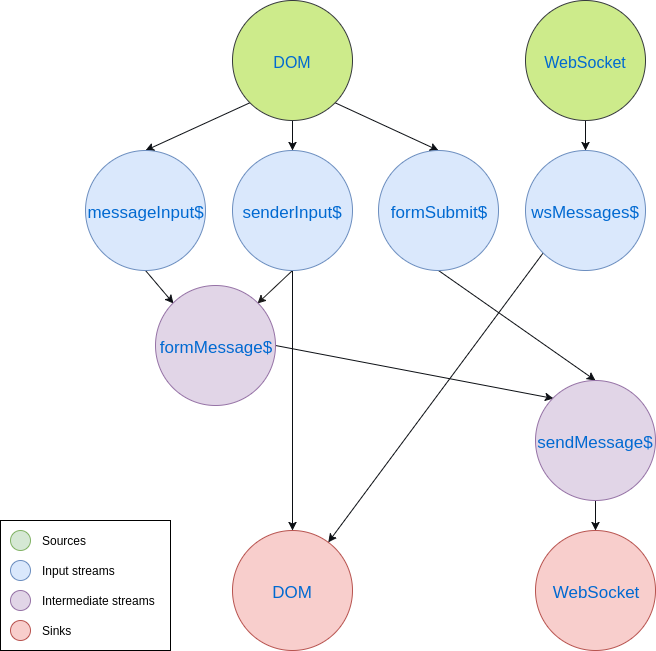
\includegraphics[width=0.7\textwidth]{chatdep}
	\caption{Dependency graph of the chat application}
	\label{figure:chat-dep}
\end{figure}

By using operators to mutate the input streams they are converted to the required format for the output streams. For the sake of readability intermediate streams are used. They are not required but are useful to make reasoning about the application easier. Finally the sinks are handled by the driver functions. The drivers will handle the I/O and side effects caused by the sinks. In the case of the chat application the DOM driver will rerender the DOM with the updated DOM and the WebSocket driver will send newly submitted messages over the WebSocket.

For elegant representation of the DOM in JavaScript JSX is used. JSX is not a templating language but rather a syntax extension to JavaScript \cite{jsx}. Because of this JSX comes with the full power of JavaScript. JSX was popularized by its use in React \cite{jsx}. In the code we provide the DOM sink as a stream of JSX objects (see listing~\ref{listing:jsx}).

\begin{lstlisting}[caption=Using JSX to define the DOM,label=listing:jsx]
function main({ DOM, ... }) { // sources in function argument
	...
	const vtree$ = Observable
		.combineLatest(wsMessages$.startWith([]), senderInput$.startWith(''))
		.map(([messages, me]) =>
			<div className="wrapper">
				<ul className="chat">
				{ messages && messages.map(m =>
					<li className={`chat__entry${me === m.sender ? ' chat__entry--mine' : ''}`}>
						<span className="chat__entry__message">{m.message}</span>
					</li>
				)}
				</ul>
			</div>
		);
		
	return { DOM: vtree$, ... }; // return sinks
}
\end{lstlisting}

In the code in listing~\ref{listing:jsx} the path towards the DOM sink in de dependency graph shown in figure~\ref{figure:chat-dep} can be recognized. The \code{wsMessages\$} and the \code{senderInput\$} streams are combined to render the current state of the application to the DOM. The \code{startWith} operators are used to define the initial state.

The JSX in listing~\ref{listing:jsx} in only an excerpt of the complete DOM. Only the logic to render the messages and determine if the message is from the sender is included. In JSX JavaScript language features are used to achieve this. To render the messages from an array of objects the \code{Array.map()} function is used. This function will map the individual messages to a JSX object. To determine if the current user is the sender of a particular message a ternary is used.

\section{Frontend with imperative programming}
\label{sec:imp-imp}

\subsection{Choice of technologies}

When developers create web applications with imperative programming they frequently use libraries such as JQuery as an abstraction over vanilla JavaScript. JQuery makes things like HTML document traversal and manipulation, event handling, animation, and Ajax simpler \cite{jquery}. While there are alternatives to JQuery like Dojo and Ext, JQuery has been and still is the most popular one by far. 

Monolithic abstractions over JavaScript like JQuery have been losing popularity in recent years because of smaller and more modular utility libraries such as lodash. New features and API's that are added to the JavaScript specification also diminish the need for JQuery. Last but not least more and more developers are migrating to more declarative frameworks and libraries to manipulate the DOM such as React.

For this application JQuery was chosen because it still sees the most usage compared to its competitors. React or Angular are not really options because they are not imperative programming frameworks.

\subsubsection{Templating language}

To render the application to the DOM it was decided to use a templating engine for convenience. Handlebars was chosen as the templating engine for the application. Handlebars provides some utility over Moustache which it is built upon. Handlebars is still a very minimal templating engine that is much lighter than popular competitors such as Pug and EJS. 

\subsection{Architecture}

The application uses a single \code{render()} function that is called whenever the application needs to rerender (see figure~\ref{figure:arch}). The application listens to events from the DOM and from the WebSocket. These events will then mutate objects that are stored in globally scoped mutable variables.

\begin{figure}[H]
	\centering
	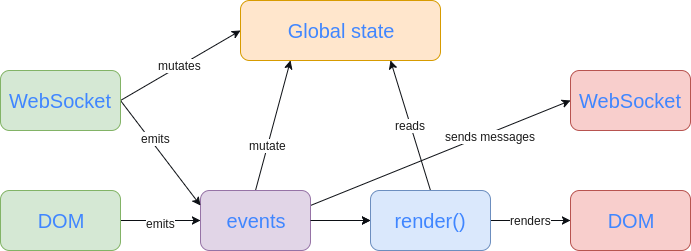
\includegraphics[width=\textwidth]{arch}
	\caption{Diagram of the imperative application architecture}
	\label{figure:arch}
\end{figure}

The event handlers from the \code{onmessage} event on the WebSocket and the \code{oninput} event from the sender input will call the \code{render()} function. Whenever the render function gets called it will read variables from the global state and rerender the application in the DOM. The onsubmit event from the message form will cause a new message to be sent over the WebSocket.

\subsection{Implementation}

This implementation uses event handlers to mutate a global state. This global state is instantiated as in listing~\ref{listing:state}.

\begin{lstlisting}[caption=The global variables that make up the application state,label=listing:state]
const template = Handlebars.compile(`
	<div class="wrapper">
		...
	</div>
`);

const messages = [];
let lastMessage = '';
let me = '';
\end{lstlisting}

The \code{messages} variable gets mutated from the \code{onmessage} event handler from the WebSocket. The \code{lastMessage} variable holds the last sent message so that it can be persisted as the input value after render. Lastly the me variable contains the current sender. This variable will be mutated by the \code{oninput}.

This application architecture is completely different from the FRP implementation. In that implementation the event streams were composed into an unidirectional dataflow (see figure~\ref{figure:chat-dep}). In this implementation event handlers are set up separately. They then all mutate global objects to communicate their data to other parts of the application. 

\subsubsection{Render function}
The \code{render()} function is implemented as shown in listing~\ref{listing:render}.
Internally the render function will compile the Handlebars template with the new data. To have the necessary data the render function first loops over the messages to check which ones are from the current user. Finally it replaces the previous version of the application in the DOM with the newly compiled Handlebars template.

\begin{lstlisting}[caption=Implementation of the render function,label=listing:render]
const render = () => {
	for (let i = 0; i < messages.length; i++) {
		const message = messages[i];
		message.isMine = message.sender === me;
	}
	const data = { messages, me, lastMessage };
	const htmlString = template(data);
	$('#app').html(htmlString);
	$('#sender').focus().val(me);
};
\end{lstlisting}

The last line of listing~\ref{listing:render} covers a corner case where the sender input loses focus while the user is typing because of the rerender. Another corner case that needed to be covered was initial render. Because the \code{render()} function only gets called from events the application would not render until an event occurs. To solve this the \code{render()} function also has to be called on load.

\section{Comparison}

In this chapter the two implementations from the section~\ref{sec:imp-frp} and section~\ref{sec:imp-imp} are compared with various metrics. First static analysis tools are used to analyze the application code. Second the performance of the two applications is compared. Finally some more subjective metrics like readability and extensibility are discussed.

\subsection{Static analysis}

\subsubsection{Bundle size}

\subsubsection{Code length}

\subsubsection{Code complexity}

\subsection{Performance}

\subsection{Readability}

\subsection{Extensibility}
\chapter*{Conclusion} % (fold)
\addcontentsline{toc}{chapter}{Conclusion}
\label{sec:besluit}

% end main content

\newpage

% references
\addcontentsline{toc}{chapter}{References}
\printbibliography[title={References},keyword={ref}]
% end references

\newpage

% bib
\addcontentsline{toc}{chapter}{Bibliography}
\printbibliography[keyword={bib}]
% end bibliography

\begin{appendices}
	\chapter{FRP frontend application logic}
	\label{appendix:frp}
	
	\begin{lstlisting}[numbers=left]
	import { Observable } from 'rxjs/Observable';
	import 'rxjs/add/observable/dom/webSocket';
	import 'rxjs/add/observable/combineLatest';
	import 'rxjs/add/operator/do';
	import 'rxjs/add/operator/map';
	import 'rxjs/add/operator/scan';
	import 'rxjs/add/operator/withLatestFrom';
	import 'rxjs/add/operator/debounceTime';
	import 'rxjs/add/operator/startWith';
	import { html } from 'snabbdom-jsx';
	
	export function App ({ DOM, ws }) {
		const wsMessages$ = ws.scan((acc, m) => [...acc, m], []);
		const formSubmit$ = DOM.select('#form').events('submit').do(e => e.preventDefault());
		const senderInput$ = DOM.select('#sender').events('input').map(e => e.target.value);
		const messageInput$ = DOM.select('#message').events('input').map(e => e.target.value);
		const formMessage$ = Observable.combineLatest(senderInput$, messageInput$)
			.map(([sender, message]) => ({ sender, message }));
		
		const sendMessage$ = formSubmit$
			.debounceTime(200)
			.withLatestFrom(formMessage$, (event, message) => JSON.stringify(message));
		const vtree$ = Observable
			.combineLatest(wsMessages$.startWith([]), senderInput$.startWith(''))
			.map(([messages, me]) =>
				<div className="wrapper">
					<ul className="chat">
					{ messages &&
					messages.map(m =>
						<li className={`chat__entry ${me === m.sender && 'chat__entry--mine'}`}>
							<img
							className="chat__entry__avatar"
							src={`https://api.adorable.io/avatars/32/${m.sender}.svg`}
							title={m.sender}
							alt={m.sender}
							/>
							<span className="chat__entry__message">{m.message}</span>
						</li>
					)}
					</ul>
					<div className="form__container">
						<form id="form" action="">
							<div className="form__inputs">
								<input className="form__input" id="sender" type="text" placeholder="Your name"/>
								<input className="form__input" id="message" type="text" placeholder="Type a message..." />
							</div>
							<div className="form__submit">
								<input className="button" type="submit" id="button__send" value="Send" />
							</div>
						</form>
					</div>
				</div>
			);
		
		return { DOM: vtree$, ws: sendMessage$ };
	}
	
	\end{lstlisting}
	
	\chapter{Imperative frontend application logic}
	\label{appendix:imp}
	
	\begin{lstlisting}[numbers=left]
	import $ from 'jquery';
	import Handlebars from 'handlebars';
	import debounce from 'lodash.debounce';
	
	Handlebars.registerHelper('equal', (val1, val2, options) => {
		val1 === val2 ? options.fn(this) : options.inverse(this);
	});
	
	$(document).ready(() => {
		const template = Handlebars.compile(`
			<div class="wrapper">
				<ul class="chat">
					{{#each messages}}
					{{#if this.isMine}}
					<li class="chat__entry chat__entry--mine">
						<span class="chat__entry__message">{{this.message}}</span>
					</li>
					{{else}}
					<li class="chat__entry">
						<img
						class="chat__entry__avatar"
						src="https://api.adorable.io/avatars/32/{{this.sender}}.svg"
						title="{{this.sender}}"
						alt="{{this.sender}}"
						/>
						<span class="chat__entry__message">{{this.message}}</span>
					</li>
					{{/if}}
					{{/each}}
				</ul>
				<div class="form__container">
					<form id="form">
						<div class="form__inputs">
							<input class="form__input" id="sender" type="text" placeholder="Your name" />
							<input class="form__input" id="message" type="text" value="{{lastMessage}}" placeholder="Type a message..." />
						</div>
						<div class="form__submit">
							<input class="button" type="submit" id="button__send" value="Send" />
						</div>
					</form>
				</div>
			</div>
		`);
		const messageWebsocket = new WebSocket('ws://localhost:8001');
		const messages = [];
		let lastMessage = '';
		let me = '';
		
		const render = () => {
			for (let i = 0; i < messages.length; i++) {
				const message = messages[i];
				message.isMine = message.sender === me;
			}
			const data = { messages, me, lastMessage };
			const htmlString = template(data);
			$('#app').html(htmlString);
			$('#sender').focus().val(me);
		};
		
		render();
		
		$('#app').on('submit', '#form', (event) => {
			event.preventDefault();
			debounce(() => {
				const message = $('#message').val();
				const sender = $('#sender').val();
				
				if (message.trim().length > 0 && sender.trim().length > 0) {
					const newMessage = { message, sender };
					lastMessage = message;
					messageWebsocket.send(JSON.stringify(newMessage));
				}
			}, 200)();
		});
		
		$('#app').on('input', '#sender', (event) => {
			me = event.target.value;
			render();
		});
		
		messageWebsocket.onmessage = (event) => {
			const message = JSON.parse(event.data);
			messages.push(message);
			render();
		};
	});
	\end{lstlisting}
	
	\chapter{Build script}
	\label{appendix:build}
	
	\begin{lstlisting}[numbers=left]
	'use strict'
	
	const fs = require('fs-extra')
	const path = require('path')
	const mkdirp = require('mkdirp')
	const webpack = require('webpack')
	const ProgressBarPlugin = require('progress-bar-webpack-plugin')
	
	const buildPath = path.join(process.cwd(), 'build')
	const publicPath = path.join(process.cwd(), 'public')
	
	mkdirp.sync(buildPath)
	
	const compiler = webpack({
		entry: [
			'./src/'
		],
		output: {
			filename: 'bundle.js',
			path: './public/'
		},
		devtool: 'source-map',
		module: {
			loaders: [
				{
					test: /\.js$/,
					loader: 'babel',
					query: {
						presets: ['es2015']
					},
					exclude: /node_modules/
				}
			]
		},
		plugins: [
			new ProgressBarPlugin(),
			new webpack.optimize.UglifyJsPlugin({minimize: true})
		]
	})
	
	compiler.run((err, stats) => {
		if (err) {
			console.log(err)
		} else {
			fs.copySync(publicPath, buildPath)
		}
	})
	\end{lstlisting}
	
	\chapter{Plato report for FRP implementation}
	\label{appendix:plato-frp}
	
	\begin{lstlisting}[numbers=left]
	{
		"summary": {
			"total": {
				"eslint": 0,
				"sloc": 58,
				"maintainability": 82.635
			},
			"average": {
				"sloc": 58,
				"maintainability": "82.64",
				"eslint": "0.00"
			}
		},
		"reports": [
			{
				"info": {
					"file": "frontend/frp-cyclejs/src/app.js",
					"fileShort": "frontend/frp-cyclejs/src/app.js",
					"fileSafe": "frontend_frp_cyclejs_src_app_js",
					"link": "files/frontend_frp_cyclejs_src_app_js/index.html"
				},
				"eslint": {
					"messages": 0
				},
				"complexity": {
					"aggregate": {
						"complexity": {
							"cyclomatic": 3,
							"cyclomaticDensity": 20,
							"halstead": {
								"bugs": 0.544,
								"difficulty": 16.056,
								"effort": 26200.817,
								"length": 252,
								"time": 1455.601,
								"vocabulary": 89,
								"volume": 1631.885,
								"operands": {
									"distinct": 72,
									"total": 136,
									"identifiers": [
										"__stripped__"
									]
								},
								"operators": {
									"distinct": 17,
									"total": 116,
									"identifiers": [
										"__stripped__"
									]
								}
							},
							"params": 11,
							"sloc": {
								"logical": 15,
								"physical": 58
							}
						}
					},
					"module": "frontend/frp-cyclejs/src/app.js",
					"maintainability": 82.635
				}
			}
		]
	}
	\end{lstlisting}
	
	\chapter{Plato report for imperative programming implementation}
	\label{appendix:plato-imp}
	\begin{lstlisting}[numbers=left]
	{
		"summary": {
			"total": {
				"eslint": 0,
				"sloc": 87,
				"maintainability": 70.429
			},
			"average": {
				"sloc": 87,
				"maintainability": "70.43",
				"eslint": "0.00"
			}
		},
		"reports": [
			{
				"info": {
					"file": "frontend/imperative/src/app.js",
					"fileShort": "frontend/imperative/src/app.js",
					"fileSafe": "frontend_imperative_src_app_js",
					"link": "files/frontend_imperative_src_app_js/index.html"
				},
				"eslint": {
					"messages": 0
				},
				"complexity": {
					"aggregate": {
						"complexity": {
							"cyclomatic": 5,
							"cyclomaticDensity": 12.821,
							"halstead": {
								"bugs": 0.524,
								"difficulty": 22.632,
								"effort": 35598.646,
								"length": 251,
								"time": 1977.703,
								"vocabulary": 77,
								"volume": 1572.963,
								"operands": {
									"distinct": 57,
									"total": 129,
									"identifiers": [
										"__stripped__"
									]
								},
								"operators": {
									"distinct": 20,
									"total": 122,
									"identifiers": [
										"__stripped__"
									]
								}
							},
							"params": 6,
							"sloc": {
								"logical": 39,
								"physical": 87
							}
						}
					},
					"module": "frontend/imperative/src/app.js",
					"maintainability": 70.429
				}
			}
		]
	}
	\end{lstlisting}
	
	\chapter{Imperative frontend application logic (vanilla JavaScript)}
	\label{appendix:vanilla}
	
	\begin{lstlisting}[numbers=left]
	const senderEl = document.getElementById('sender');
	const messageEl = document.getElementById('message');
	const messageListEl = document.getElementById('chat');
	const formEl = document.getElementById('form');
	const messageWebsocket = new WebSocket('ws://localhost:8001');
	const messages = [];
	let me = '';
	
	const debounce = (func, wait) => {
		let timeout;
		return () => {
			let context = this, args = arguments;
			const later = () => {
				timeout = null;
				func.apply(context, args);
			};
		
			clearTimeout(timeout);
			timeout = setTimeout(later, wait);
		};
	};
	
	const createSenderAvatar = (sender) => {
		const avatarImg = document.createElement('img');
		avatarImg.classList.add('chat__entry__avatar');
		avatarImg.src = `https://api.adorable.io/avatars/32/${sender}.svg`;
		avatarImg.title = sender;
		avatarImg.alt = sender;
		
		return avatarImg;
	};
	
	const createMessageSpan = (message) => {
		const messageSpan = document.createElement('span');
		messageSpan.classList.add('chat__entry__message');
		const messageText = document.createTextNode(message);
		messageSpan.appendChild(messageText);
		
		return messageSpan;
	};
	
	const createMessage = (message) => {
		const messageLi = document.createElement('li');
		const currentSender = senderEl.value;
		const isMine = currentSender === message.sender;
		const classes = isMine ? ['chat__entry', 'chat__entry--mine'] : ['chat__entry'];
		messageLi.classList.add(...classes);
		
		if (!isMine) {
			const avatarImg = createSenderAvatar(message.sender);
			messageLi.appendChild(avatarImg);
		}
		
		const messageSpan = createMessageSpan(message.message);
		messageLi.appendChild(messageSpan);
		return messageLi;
	};
		
	const addMessage = (message) => {
		const messageLi = createMessage(message);
		messageListEl.appendChild(messageLi);
	};
	
	const onSubmitDebounced = debounce((event) => {
		const message = messageEl.value;
		const sender = senderEl.value;
		
		if (message.trim().length > 0 && sender.trim().length > 0) {
			const newMessage = { message, sender };
			messageWebsocket.send(JSON.stringify(newMessage));
		}
	}, 200);
	
	formEl.addEventListener('submit', onSubmitDebounced);
	formEl.addEventListener('submit', (event) => {
		event.preventDefault();
	});
	
	senderEl.addEventListener('input', (event) => {
		const newSender = event.target.value;
		const notMyMessagesIndexes = [];
		const myMessagesIndexes = [];
		
		if (newSender.trim() !== me) {
			for (let i = 0; i < messages.length; i++) {
				const message = messages[i];
				if (message.sender === me) {
					const messageLi = messageListEl.childNodes.item(i);
					messageLi.classList.remove('chat__entry--mine');
					messageLi.insertBefore(createSenderAvatar(message.sender), messageLi.firstChild);
				} else if (message.sender === newSender) {
					const messageLi = messageListEl.childNodes.item(i);
					messageLi.classList.add('chat__entry--mine');
					messageLi.removeChild(messageLi.firstChild);
				}
			}
		}
		me = newSender.trim();
	});
	
	messageWebsocket.addEventListener('message', (event) => {
		const message = JSON.parse(event.data);
		messages.push(message);
		addMessage(message);
	});
	\end{lstlisting}
	
	\chapter{Plato report for vanilla JavaScript implementation}
	\label{appendix:plato-vanilla}
	
	\begin{lstlisting}[numbers=left]
	{
		"summary": {
			"total": {
				"eslint": 0,
				"sloc": 106,
				"maintainability": 69.146
			},
			"average": {
				"sloc": 106,
				"maintainability": "69.15",
				"eslint": "0.00"
			}
		},
		"reports": [
			{
				"info": {
					"file": "src/app.js",
					"fileShort": "src/app.js",
					"fileSafe": "src_app_js",
					"link": "files/src_app_js/index.html"
				},
				"eslint": {
					"messages": 0
				},
				"complexity": {
					"aggregate": {
						"complexity": {
							"cyclomatic": 9,
							"cyclomaticDensity": 11.538,
							"halstead": {
								"bugs": 1.062,
								"difficulty": 33.103,
								"effort": 105486.821,
								"length": 469,
								"time": 5860.379,
								"vocabulary": 111,
								"volume": 3186.581,
								"operands": {
									"distinct": 87,
									"total": 240,
									"identifiers": [
										"__stripped__"
									]
								},
								"operators": {
									"distinct": 24,
									"total": 229,
									"identifiers": [
										"__stripped__"
									]
								}
							},
							"params": 10,
							"sloc": {
								"logical": 78,
								"physical": 106
							}
						}
					},
					"module": "src/app.js",
					"maintainability": 69.146
				}
			}
		]
	}
	\end{lstlisting}
\end{appendices}

\end{document}
